% general
\documentclass[a4paper,12pt]{article}

% other packages
\usepackage[fleqn]{amsmath}

\usepackage{geometry}
\geometry{a4paper, portrait, margin=0.9in}

% graphics
\usepackage{graphicx}
\graphicspath{{./plots/}}
\usepackage[font=small,labelfont=bf]{caption}
\usepackage{float}
\newcommand{\indep}{\rotatebox[origin=c]{90}{$\models$}}

% landscape and longtables
\usepackage{pdflscape}
\usepackage{longtable}

\usepackage{sectsty}

% hebrew
\usepackage{fontspec}
\usepackage{polyglossia}
\usepackage[utf8x]{inputenc}
%\usepackage{hebfont}
%\newfontfamily\hebrewfont[Script=Hebrew]{Miriam Mono CLM}
%\newfontfamily\hebrewfont[Script=Hebrew]{Frank Ruehl CLM}
\newfontfamily\hebrewfont[Script=Hebrew]{David CLM}
\newfontfamily{\hebrewfontsf}[Script=Hebrew]{Linux Libertine O}
\newfontfamily{\hebrewfonttt}[Script=Hebrew]{Linux Libertine O}

% Font experiments
%\setmainfont{DejaVu Sans}
%\setmonofont{DejaVu Sans}
%\newfontfamily\hebrewfont{DejaVu Sans}[Script=Hebrew]
%\newfontfamily\hebrewfontsf{DejaVu Sans}[Script=Hebrew]
%\newfontfamily\hebrewfonttt{DejaVu Sans}[Script=Hebrew]

\setmainlanguage{english}
\setotherlanguage{hebrew}

% bib
\usepackage[backend=bibtex, sorting=none]{biblatex}
\addbibresource{bibtex/proposal.bib}

% spacing
\usepackage{setspace}
\linespread{1}
\setlength{\parskip}{\medskipamount}
\setlength{\parindent}{0pt}

% appendices
\usepackage[toc,page]{appendix}

% csv
\usepackage{csvsimple}

\begin{document}

	\begin{titlepage}
		\centering
		{\scshape\LARGE Ben-Gurion University of the Negev\par}
		\vspace{1cm}
		{\Large PhD Proposal\par}
		\vspace{2cm}
		{\huge\bfseries Improving Cardiovascular Disease Prediction\par}
		\vspace{1cm}
		\begin{hebrew}
		{\huge\bfseries שיפור חיזוי מחלה קרדיווסקולרית\par}
		\end{hebrew}
		\vspace{1.5cm}
		{\Large\itshape Noam Barda, MD\par}
		{\large \today\par}
		\vfill
		Supervisor's Signature, Prof. Nadav Davidovich: \underline{\hspace{5cm}}\par
		\vspace{0.5cm}
		Supervisor's Signature, Prof. Eitan Bachmat: \underline{\hspace{5cm}}\par
		\vspace{0.5cm}
		Chairman of Departmental Graduate Studies's Signature: \underline{\hspace{5cm}}\par
		
	\end{titlepage}
	
	\tableofcontents
	\newpage
	
	\section{Abstract}
	
		\subsection{Background}
		
		Cardiovascular disease (CVD), including myocardial infarction (MI) and cerebrovascular accident (CVA), remains a significant cause of morbidity and mortality\cite{ODonnell2016} worldwide, despite reduced incidence in the developed world in recent years\cite{Koton2014,Vangen-Loenne2017}.
		
		Since the early 1990s, and more so in the last few years,  multivariable risk prediction models have been created to estimate patients' risk for cardiovascular disease (e.g. \cite{Wilson1998,Conroy2003,DAgostino2008}). These models are used to identify patients at risk and are capable of exact risk quantification over time\cite{Goff2014}. Through their many variations, these risk models are included in different guidelines and occupy an important place in prevention of CVD\cite{Goff2014}.
	
		Given this central place, improvement of cardiovascular disease prediction models has the potential to greatly impact public health.
		
		\subsection{Goals}
		
		In this thesis we will explore three ways to improve CVD prediction. First, we will examine the incorporation of novel biomarkers, generated through automated algorithms, into the model. Second, we will examine A novel way to generate prediction models that does not require any domain expertise, and has the potential to better select variables and construct models. Lastly, we will examine the use of causal inference methods to better quantify the effect of patient risk-lowering interventions.

		\subsection{Methods}
		
		The baseline model used will be the 2013 American Heart Association/American College of Cardiology (AHA/ACC) pooled cohort equations\cite{Goff2014}. This model is of great importance, and is used in the AHA/ACC guidelines and the United States Preventive Services Task Force (USPSTF) guidelines for CVD prevention\cite{Bibbins-Domingo2016}. The population of all studies is the general population of Clalit Health Services (CHS), the largest sick fund in Israel.
		
		We will first employ automated coronary calcium scores in an attempt to improve the prediction. These scores will be generated automatically from existing chest CT scans via a computer vision machine learning algorithm. Next, We will construct an automatic generic algorithm to generate prediction models using little-to-none human intervention. This algorithm will extract variables from the database, choose the most relevant ones and construct a model while performing hyperparameter tuning. Lastly, We will use causal inference techniques for estimating the Average Treatment Effect (ATE) and Individual Treatment Effect (ITE) to estimate the effect of intervening on different patient characteristics.
		
		\subsection{Importance}
		
		CVD prediction is crucial for CVD prevention. All methods suggested in this thesis hold a promise for improving CVD prediction and allowing better tailoring of intervention techniques.
		
		\subsection{Keywords}
		
		Medical Prediction Models, Generic Prediction, Computer Vision, Cardiovascular Disease, Electronic Health Records, Causal Inference
	
	\begin{hebrew}	
	\section{\texthebrew{תקציר בעברית}}
	
		\subsection{\texthebrew{רקע}}
		
		מחלה קרדיווסקולרית, הכוללת אוטם לבבי ושבץ מוחי, עודה סיבה מובילה לחולי ותמותה\cite{ODonnell2016} ברחבי העולם, וזאת חרף ירידה בהיארעותה בעולם המערבי בשנים האחרונות\cite{Koton2014,Vangen-Loenne2017}.

				מתחילת שנות ה-90 החלה, ובשנים האחרונות גברה, יצירתם של מודלים רב-משתניים לחישוב סיכון למחלות שונות(לדוגמה \cite{Wilson1998,Conroy2003,DAgostino2008}). מודלים אלו משמשים לזיהוי חולים בסיכון, ומאפשרים כימות מדויק של הסיכון לאורך שנים רבות\cite{Goff2014}. כיום, בצורותיהן השונות, מודלים אלו כלולים בקווים המנחים של ארגונים מקצועיים רבים, ולהם מקום חשוב הן במניעה הראשונית והן באבחנה של מחלות \cite{Graham2007,Goff2014}.
				
				בהינתן חשיבותן הרבה זו, לשיפור הביצועים של מודלי חיזוי הפוטנציאל להשפיע עמוקות על בריאות הציבור.
			
		\subsection{\texthebrew{מטרות}}
		
				בתזה זו אנו מתכוונים לחקור שלושה דברים לשיפור חיזוי מחלה קרדיוסקולרית. בתחילה, אנו נבדוק האפקט של שילוב ביומרקרים חדשניים, הנוצרים ע"י אלגוריתמים אוטומטיים, לתוך מודל החיזוי. לאחר מכן, אנו נחקור דרך חדשנית לבניית מודלי חיזוי אשר אינה דורשת היעזרות במומחי תוכן מהתחום, ולה הפוטנציאל לבחירת משתנים ומודל טובים יותר. לבסוף, אנו נחקור השימוש בשיטות מתחום ההסקה הסיבתית על מנת לכמת ההשפעה של התערבויות שונות להפחתת הסיכון.
				
		\subsection{\texthebrew{שיטות}}
		
		המודל הבסיסי בו נעשה שימוש בעבודה זו הוא מודל האגודה האמריקאית למחלה לב משנת 2013\cite{Goff2014}. למודל זה חשיבות רבה, והוא משמש בקווים המנחים למניעת מחלה קרדיווסקולרית של האגודה האמריקאית למחלות לב ושל הצוות האמריקאי לשירותים מניעתיים\cite{Bibbins-Domingo2016}. האוכלוסיה בכל המחקרים תהיה אוכלוסיית המבוטחים של קופת החולים כללית, הקופה הגדולה בישראל.
		
		בתחילה נשתמש בניקוד לכמות הסידן בעורקי הלב על מנת לשפר החיזוי. ניקוד זה יופק באופן אוטומטי ב-CT חזה קיימים באמצעות אלגוריתמי למידת מכונה לראיה ממוחשבת. לאחר מכן אנו נבנה אלגוריתם אוטומטי אשר תפקידו לייצר מודלי חיזוי עם מינימום התערבות אנושית. אלגוריתם זה ישלוף המשתנים מבסיס הנתונים, יבחר הרלוונטיים מהם ביותר ויבנה מודל תוך ביצוע טיוב לפרמטרים. לבסוף, אנו ניעזר בטכניקות של הסקה סיבתית על מנת להעריך האפקט הממוצע והאישי של התערבויות שונות בפרט להפחתת סיכון קרדיווסקולרי.

		\subsection{\texthebrew{חשיבות}}
		
		חיזוי מחלה קרדיווסקולרית חיונית למניעתה. לכל השיטות המתוארות בעבודה זו היכולת לשפר חיזוי מחלה קרדיווסקולרית ולאפשר החלטות מושכלות יותר בנוגע למניעה. 
			
			\subsection{\texthebrew{מילות מפתח}}
			
			מודלי חיזוי רפואיים, חיזוי גנרי, ראיה ממוחשבת, מחלה קרדיווסקולרית, תיק רפואי ממוחשב, הסקה סיבתית.
		
	\end{hebrew}
	
	\section{Aim of the Thesis}
	
	The main aim of this thesis is to examine different methods of improving cardiovascular disease risk prediction.
	
	Three methods will be explored:
	\begin{description}
		
		\item[Use of Automatically Generated Biomarkers] We will examine the effect of incorporating into the model a novel biomarker based on the coronary calcium score. This biomarker will be automatically generated using a machine learning algorithm from existing chest CTs.
		
		\item[Generic Risk Prediction] A modern and novel approach to develop risk models based on Electronic Health Record (EHR) data will be developed. The full details of this approach will be detailed below, under "Research Methodology", but briefly, it will require no preliminary domain expertise, instead utilizing modern methods to simultaneously choose variables and create the model based on them.
		
		\item[Determining Intervention Effects] CVD Prediction models are often used to decide on interventions designed for disease prevention. But by themselves, these models give no information regarding the relative efficacy of such interventions. We will utilize methods designed for causal inference to estimate the expected effect of such interventions at the patient level.
		
	\end{description}
	
		Based on these aims, we hypothesize:
		\begin{enumerate}
			
			\item That automatically generated biomarkers from existing scans will improve CVD prediction with no patient harms.
			
			\item That using less pre-specification of risk factors, and allowing a computerized algorithm to select risk factors in an autonomous fashion, will enable detection of novel risk factors, whose inclusion in future risk models will improve their performance.
			
			\item That causal inference methods can be used to estimate not only a patient's risk, but also the change in risk given certain interventions.
			
		\end{enumerate}
		
	\section{Importance and Background}
	
		We will survey the pertinent background in general and then for each step in turn, highlighting the gap in existing knowledge to which we seek to contribute.

		\subsection{General Background}
		
			\subsubsection{Epidemiology of Cardiovascular Disease and Stroke}
			
			In its usual definition, cardiovascular disease (CVD) includes several disease categories\cite{WHO2017}:
			\begin{enumerate}
				\item Coronary Heart Disease
				\begin{enumerate}
					\item Myocardial Infarction
					\item Angina Pectoris
					\item Heart Failure
					\item Coronary death
				\end{enumerate}
				\item Cerebrovascular Disease
				\begin{enumerate}
					\item Stroke (Thrombotic and Hemorrhagic)
					\item Transient Ischemic Attack
				\end{enumerate}
				\item Peripheral Artery Disease
				\item Aortic Disease
				\begin{enumerate}
					\item Atherosclerosis
					\item Aneurysm
				\end{enumerate}
				\item Rheumatic Heart Disease
				\item Congenital Heart Disease
				\item Venous Thromboembolism
				\begin{enumerate}
					\item Pulmonary Embolism
					\item Deep Vein Thrombosis
				\end{enumerate}
			\end{enumerate}
			
			CVD is very common. Lifetime risk for people aged 30 with no prior cardiovascular disease approaches 50 percent\cite{Rapsomaniki2014}, with coronary heart disease being the most common specific diagnosis\cite{Benjamin2017}.
			
			While the rates of cardiovascular disease have declined in developed countries over the last 30 years\cite{Koton2014,Vangen-Loenne2017}, they remain significant public health problems, being the second most common cause of mortality and third most common cause of disability worldwide\cite{Lozano2012}. The statistics in Israel are similar\cite{ICDC2017}.
			
			Among diseases with such a significant public health impact, cardiovascular disease stands out in two ways. First, its risk factors are well understood, with 90\% of its population-attributable-risk caused by nine risk factors. It's also a very preventable disease, as these risk factors are mostly preventable\cite{Yusuf2004,ODonnell2016}: Smoking, dyslipidemia, hypertension, diabetes, etc.
			
			\subsubsection{History of multivariable Risk Models}
			
			These unique characteristics have made CVD the main outcome in risk models, when such models began to enter clinical practice in the 1990s\cite{Wilson1998,NationalCholesterolEducationProgramNCEPExpertPanelonDetection2002,Conroy2003,Hippisley-Cox2007,DAgostino2008,Hippisley-Cox2008,Goff2014}. Still the most notable of said risk models is the Framingham risk model family, developed on a US population in Massachusetts, Boston\cite{Wilson1998}, and the SCORE risk model, developed in 2003 on a European population\cite{Conroy2003}.
			
			Perhaps more important that their mere existence, is that these models have made their way into widely-accepted international guidelines, with their use mandated in routine clinical care. Two examples we'll cite are the use of these risk models in deciding on Statin therapy\cite{Goff2014} and their use in deciding on anti-platelet therapy\cite{Bibbins-Domingo2016}, both for primary prevention of CVD.
			
			While CVD prediction was the bedrock for clinical risk models, they have since spread to encompass a large variety of diseases categories\cite{Kanis2008,Kansagara2011}, and have found use not only in prediction, but also in diagnosis\cite{Usher-Smith2016}. This increasingly important place taken by risk models has brought about the publication of guidelines designed to regulate and improve their creation\cite{Collins2015}. As estimating the probability for existing and future disease is a significant portion of the clinical process\cite{Moons2009}, and as this task can in large parts be automated, it seems likely that risk models will gain an increasingly important place in the medical practice.
			
			\subsubsection{Limitations of Risk Models}
			
			Naturally, risk models are developed on a specific population, whose data is available to the researchers developing the model. As patients differ in a variety of ways (both genetic and environmental), and even such basic things as lab methods and disease definitions differ in different areas, models tend to function better when used on the population on which they were developed\cite{DAgostino2001,Bastuji-Garin2002}.
			
			Recent models have tried to deal with this problem by including more ethnically varied populations\cite{DeFilippis2015} or recalibrating the model for each new population\cite{Kanis2008}, but such efforts are limited to specific risk models, and even then have only been partially successful\cite{Dagan2017}. As one specific Israeli example, this phenomenon was observed in a recent publication that illustrated significant mis-calibration for osteoporosis prediction models that are in wide clinical use and incorporated into guidelines\cite{Dagan2017}. As the probabilities generated by the model eventually help determine the proper interventions to perform, according to respective guidelines, such mis-calibration could invalidate the use of the model, making external validation an important endeavor\cite{Moons2012}.
			
		\subsection{Part I}
		
			\subsubsection{Coronary Artery Calcium}

			Atherosclerotic disease is the main cause of CVD. As sclerotic plaques in the arteries bind calcium, which in turn is visible on imaging studies, quantification of coronary artery calcium (CAC) via CT scans can be used to quantify the extent of atherosclerotic disease in the coronary arteries. It has been demonstrated that such CAC quantification can help guide medical therapy and lifestyle modification choices\cite{Takx2015,Elias-Smale2010,Erbel2010,Vliegenthart2005,Becker2005}.
			
			Traditionally, CAC scoring has required a dedicated electrocardiogram (ECG)-gated cardiac computed tomography (CT) scan performed with and without intravenous contrast at significant financial costs\cite{Halpern2010}. More recently, several studies have demonstrated good inter-technique concordance for CAC scoring on low-dose, non-gated chest CTs as compared to dedicated, contrast-enhanced and ECG-gated cardiac CTs\cite{Wu2008,Budoff2011}.
			
			\subsubsection{Integration of CAC Scores into CVD Prediction Models}
			
			On the one hand, it has been shown that integrating CAC scores into existing CVD prediction models yields more accurate predictions\cite{Polonsky2010,Greenland2004}. On the other hand, obtaining a CAC score requires human radiologist time for scoring and dedicated CT scans, with their associated radiation exposure and monetary costs. Weighting these benefits and harms, a recent USPSTF statement recommends against the routine incorporation of CAC scores into CVD prediction models\cite{Force2018}.
			
			\subsubsection{Medical Computer Vision}
			
			With the fairly recent rise of deep neural networks, computer performance in vision tasks has risen enormously, and can rival human performance on many tasks. Specifically in the medical field, such neural network-based algorithms are now used to diagnose fractures\cite{Lindsey2018}, to review pathology slides\cite{EhteshamiBejnordi2018} and to assist in pneumonia diagnosis\cite{Abiyev2018}, among other things. To be trained, these algorithms require annotated data, usually annotated by a human specialist; but once trained, these algorithms require no further human involvement.
			
			\subsubsection{Automatic CAC Scoring}
			It has recently been shown that reliable CAC scoring can be obtained algorithmically from low dose chest CT data\cite{Isgum2012,Shadmi2018} and that such measurements were correlated with cardiovascular events in a cohort of individuals undergoing CT screening for lung cancer\cite{Takx2015a}. It has not been demonstrated if such automated scores are capable of improving on existing multivariable risk prediction models\cite{Force2018}.
			
			\subsubsection{The Scientific Gap}
			CAC scores have proven utility for CVD prediction, but obtaining them involves harms that are often unacceptable. Such harms are non-existent when the CAC score is obtain automatically from existing CT scans. We will evaluate the improvement to existing prediction algorithms when such automatically obtained CAC scores are integrated into the model.
			
		\subsection{Part II}
		
			\subsubsection{Methodology of Traditional Risk Models}
		
			For traditional medical risk models, two design decisions are ubiquitous\cite{Weng2017}:
			\begin{enumerate}
				\item They are based on traditional biostatistical methodology such as generalized linear and cox models.
				\item They rely heavily on the use of domain expertise to identify relevant risk factors.
			\end{enumerate}
		
			Informally described, we could say that the model is tasked to estimate the relative weights of risk factors, themselves independently pre-identified by domain experts.
		
			\subsubsection{Generalized Linear Models}
			
			Generalized linear models (GLMs) are parametric models that are generalizations of ordinary linear regression, allowing outcome variables to have non-normal error distributions\cite{Nelder1972}.
			
			While classic linear regression follows the form:
			\begin{equation*}
			E[Y] = x^t \beta
			\end{equation*}
			
			GLMs have the form:
			\begin{equation*}
			E[Y] = g^{-1} (x^t \beta)
			\end{equation*}
			
			With g being the link function connecting the linear predictor space with the outcome space.
			
			For example, logistic regression uses the logit function as the link, $ \mu = \frac{\exp (x^t \beta)}{1 + \exp (x^t \beta)} $, while linear regression uses the identity function.
			
			The model then uses a loss function, usually maximum likelihood, to estimate the coefficients of the model. Under certain assumptions, these coefficients can have epidemiological interpretations, such as the coefficients of logistic regression being interpreted as the odds ratio of an exposure for a given outcome. The model can also be used for prediction, disregarding all such assumptions.
			
			\subsubsection{Cox Proportional Hazards Model}
			
			The cox model is a survival analysis model (that is, it uses a compound outcome of time-to-event data) that is semi-parametric. A baseline hazard ($ \lambda_0 $) is estimated non-parametrically from the data, while a parametric linear hazard model is estimated in parallel\cite{Cox1972}.
			
			The overall hazard model is thus $ \lambda(t) = \lambda_0(t) \cdot x^t \beta $. The hazard itself is a somewhat elusive term rooted in calculus, representing the probability of death at a certain infinitesimal time window assuming survival up to that point. Survival is then one minus the integral of the hazard over time.
			
			Similar to GLMs, the coefficients are estimated using a process of maximum likelihood (dubbed partial likelihood in the context of Cox regression), and under strict assumptions have the interpretation of hazard ratios, similar to odds ratios.
			
			The assumptions for cox regression warrant special mention. While the assumption of linearity is similar to GLMs, cox regression also assumes proportionality - that is, that the hazard ratio between risk factors remains constant over time. This is a very strong assumption that does not always hold. Some models circumvent this assumption at the cost of complexity and loss of interpretability. Just as before, the model can also be used for prediction, disregarding all assumptions.
			
			\subsubsection{Parametric Vs. Non-Parametric Models}
			Parametric models, such as those described above, summarize the data with a set of parameters of fixed size that is independent of the number of training examples. This has the advantage of simplicity, interpretability and speed, but also leads to biases in prediction if the "true" population model is different than the chosen model.
			
			Non-parametric models make no such assumptions about the structure of the target function they seek to learn. This requires far more data for accurate training, and does not allow interpretation of coefficients using terms such as odds ratios, but does afford more predictive accuracy when sufficient data exists\cite{Russell2002}.
			
			\subsubsection{The Rise of AI and Machine Learning}
		
			In recent years the fields of machine and statistical learning have seen a tremendous rise\cite{Obermeyer2016}. this growth in machine learning, including predictive modeling, has occurred thanks to three main factors\cite{Shalev-Shwartz2014}:
			\begin{itemize}
				\item A large increase in the amount of accessible data.
				\item The development of new algorithms and methods.
				\item An increase in computation power.
			\end{itemize} 
			These new methods have several defining characteristics, including:
			\begin{itemize}
				\item The use of a wider range of algorithms, not limited to generalized linear models.
				\item Less reliance on domain expertise, in essence allowing the algorithm to both find the main risk factors and to estimate their respective weights.
				\item The need for larger sample sizes, to allow the more complex modeling to occur successfully.
			\end{itemize}
			To date, these methods have yet to gain wide-acceptance in medical practice\cite{Obermeyer2016,Deo2015}.
			
			\subsubsection{Black-Box Vs. White-Box Models}
			While there are obstacles from many different domains to the integration of machine learning approaches in medicine: psychological, legal, regulatory and others, one overarching concern is the preeminence of black-box models in machine learning\cite{Price2015}.
			
			Broadly defined, black-box models are models whose results cannot be readily explained. For example, a logistic regression result can be fairly easily reasoned about: baseline risk was x\%, and a certain combination of variables increased the risk by y\% more. The same cannot be said for most models used in modern machine learning, including neural networks and tree-ensemble models. These models generate a result that is a complex non-linear function of their inputs, and one cannot easily explain why a specific patient got a risk of x\%, while another got y\%.
			
			Beyond the legal and psychological difficulty this creates (how does one explain, to oneself and others, a decision based on unclear reasoning?), it also introduces the possibility of discrimination. The algorithm could choose to optimize for one (majority) population, while neglecting other (minority) populations\cite{Hebert-Johnson2017}. This fascinating area of research falls under the more general notion of algorithmic fairness, more widely studied in other non-medical fields\cite{Corbett-Davies2017}, and is beyond the scope of this thesis.
			
			\subsubsection{Electronic Health Record based Observational Studies}
		
			Most medical risk models in wide-use were developed based on specialized cohort studies\cite{Goldstein2016}. This has the known advantages of cohort studies, most notably the accurate definition of exposures and outcomes, but is expensive and time-consuming, and by definition only allows inclusion of risk factors that were decided on in advance and measured as part of the study. On the other hand, with the larger availability of EHRs, risk models developed on such data have risen in amount. These models have the known disadvantages of EHR data (first of which are the non-standardized definitions), but offer a wealth of information that in certain cases, including the case in Israel\cite{Lovis2015}, encompasses the full extent of a patient's encounters with the health system\cite{Goldstein2017}.
			
			\subsubsection{The Scientific Gap}
			
			We suggest using the unique availability of widely encompassing EHR data with large historic depth, coupled with modern statistical learning methods, to develop a generic method for generation of risk models based on the Clalit's EHR.
			
			This method will make use of most available EHR data, and will require no pre-specification of risk factors, instead allowing the algorithm to ascertain the relative importance of the different factors by itself. Not only will this allow the creation of accurate risk models, it will also provide a way to automatically identify associations that exist in the EHR and could represent novel risk factors and biological pathways.
			
			We will then use this method to develop a specific model to predict cardiovascular disease. As this model will make use of large portions of the EHR data and will be purposely built on the Clalit's population, it is likely to perform well.
		
		\subsection{Part III}
		
			\subsubsection{Aim of Risk Models}
			
			Invariably, the aim of prediction is prevention. CVD carries a high burden of mortality and morbidity, but as its risk factors are well mapped\cite{Yusuf2004}, steps can be taken to mitigate the risk. But - deciding on proper interventions requires knowledge of not only the absolute risk, but also the relative effectiveness of the different possible interventions. Coupled with the harms, this allows proper decision making.
			
			\subsubsection{Correlation is not Causation}
			
			By themselves, predictive models do not give any information regarding the expected effect of any change. Predictive models model the probability of the outcome given the covariates, and contain no direct information regarding the effect of changing any such covariate.
			
			Mathematically, given outcome $ Y $, covariate vector $ X $ and treatment $ T $, predictive models model
			
			\begin{equation*}
			E[Y|X,T]
			\end{equation*}
			And a subtracting the predictions with the treatment in different states yields us
			\begin{equation*}
			E[Y|T=1] - E[Y|T=0]
			\end{equation*}
			This is, in general, not equal to the causal effect of T on Y, which is defined as
			\begin{equation*}
			E[Y^1] - E[Y^0]
			\end{equation*}
			Where $ Y^i $ is the counterfactual for $ T=i $.
			
			That is to say, correlation is not causation. Regardless, knowledge of the absolute risk without knowledge of the relative effects of different interventions is not sufficient for deciding on interventions.
			
			\subsubsection{Causal Inference}
			In general, the individual treatment effect (ITE) for a specific patient, $ Y_i^1 - Y_i^0 $ can never be known, as one of the counterfactuals will always be hidden. But, under certain assumptions, the average causal effect is identifiable from observational data.
			\begin{description}
				\item[Ignorability] Given the covariates, the outcome is independent of the treatment: $ Y \indep  T | X$
				\item[Positivity] The probability of treatment is positive for any vector of covariate values: $ P(T = 1|X) > 0 $
				\item[Consistency] The intervention is well defined, and exposes the matching counterfactual value: $ P(Y^i) = P(Y|T=i) $
			\end{description}
		
			Under these assumptions, the causal effect can be identified using a variety of methods, well known to epidemiologists (i.e. covariate adjustment, inverse probability weighting, matching). When this effect is estimated conditional on certain values for X, we derive the Conditional Average Treatment Effect (CATE, $ E[Y_1|X] - E[Y_0|X] $), which is a useful surrogate for the ITE.
			
			Knowledge of a patient's absolute prediction for CVD, together with the relative individualized expected benefit for the patient would allow optimal decision making.
			
			\subsubsection{The Scientific Gap}
			
			We suggest that a predictive model coupled with conditional average treatment effects is a far more powerful tool than just predictions. We are not aware of any such tools in existence. Such a tool would allow both better decisions by the physician and would motivate the patient to reduce his risks, with full knowledge of the expected benefit.
			
	\section{The Novelty of the Thesis}
	
	All aforementioned aspects of the thesis contain measures of novelty to them:
	
	\begin{itemize}
		
		\item[Use of Automatically Generated Biomarkers] Use of existing studies (imaging or otherwise) to derive biomarkers with predictive power could be of great use to patients, who would benefit from more accurate prediction. The automation of the process would also render it feasible for implementation.
		
		\item[Generic Risk Prediction] We propose that the methodology by which the model will be developed, and specifically its wide applicability, requiring little human intervention and pre-processing, offers significant advantages. The ability to identify risk factors and construct models for a wide variety of pathologies, some of which "unmapped" in regard to their primary risk factors, offers a promise of better understanding and more focused interventions to prevent these diseases.
		
		\item[Determining Intervention Effects] To date, predictive models have focused on prediction alone. While this is useful, it is not the entire picture, and modeling the treatment effects is of paramount importance for better physician and patient decision making.
		
	\end{itemize}
	
	\section{Published Work}
	
	The epidemiological characteristics of CVD in general and of stroke in particular are well understood\cite{Koton2014,Vangen-Loenne2017}, and the dominant risk factors in the population well mapped\cite{Yusuf2004,ODonnell2016}. This is true both in the developed and in the developing world\cite{Lozano2012}. It is also true in Israel\cite{ICDC2017}.
	
	The increasingly central role filled out by risk prediction models in medicine has been observed\cite{Moons2009}, as have the challenges of developing such models based on Electronic Health Record (EHR) data\cite{Goldstein2016,Goldstein2017}. This rapid rise in the number of risk prediction models has led to the writing of specific guidelines on how to develop such risk models and report their results\cite{Collins2015}.
	
	Many CVD risk models have been developed in the last 30 years, most prominent of which are the Framingham\cite{Wilson1998,NationalCholesterolEducationProgramNCEPExpertPanelonDetection2002,DAgostino2008,Goff2014}, SCORE\cite{Conroy2003} and Qrisk\cite{Hippisley-Cox2007,Hippisley-Cox2008} families of models.	Two of these model families also offer a stroke-specific model\cite{Wolf1991,DAgostino1994,Hippisley-Cox2013}.
	
	Risk models have been incorporated into guidelines for the prevention, diagnosis and treatment of varying conditions. Specifically for CVD prediction, these risks help decide on cholesterol lowering treatment, anti-platelet treatment and more generally, the intensity of follow-up\cite{NationalCholesterolEducationProgramNCEPExpertPanelonDetection2002,Graham2007,Goff2014,Bibbins-Domingo2016}.
	
	The utility of CAC is well known\cite{Erbel2010}, and the debate regarding its use ongoing\cite{Greenland2018}. Attempts to automatically derive it have been published \cite{Isgum2012,Shadmi2018} and tested for correlations with the outcome \cite{Takx2015}, but never assessed for yield beyond the the existing state-of-the-art model\cite{Force2018}.
	
	Much has been written on the advent of AI in general and machine learning in particular. In a relatively short time span, these technologies have penetrated large parts of the domains of modern life, and continue to do so with increasing force\cite{Ng2017}.
	
	That this process has been relatively slow in medicine is also widely recognized, and many efforts now exist to better incorporate such technologies in health-care\cite{Obermeyer2016}. Specifically for risk prediction models, recent literature has emerged that details attempts at developing more generic risk models, though different than the idea proposed here both in method and in goal\cite{Rajkomar2018}.
	
	Causal inference is not a new methodology \cite{GuidoW.Imbens2015,StephenL.Morgan2015}, but has been garnering much attention lately\cite{JudeaPearl2018}. While many calculators are published online, allowing patients to modify their risk factors (i.e. \cite{NHS2016}), none that we know of incorporates causal inference.
	
	\section{Research Methodology}
	We will divide this section into two parts. In the first part, we'll review important concepts that will be used in the analysis. In the second part, we'll detail the exact research plan for this thesis per each part.
	
	\subsection{Important Concepts}
	
		\subsubsection{Source of Data for Study}
		The general population for all different parts of the study is the population of patients insured by Clalit Health Services (CHS). CHS is the largest sick fund in Israel, with an insured population of 4.5 active members. Clalit is both an insurer and a provider, directly providing primary care, specialist care, lab, imaging and pharamacy services. Additionally, clalit directly operates several large hospitals. The “attrition rate” (the percentage of patients leaving the sick fund each year) stands on less than 2\%, allowing long term follow-up of patients.
		
		The data will be collected using the CHS's electronic health record (EHR). CHS has maintained a comprehensive electronic health record since the year 2000, and has continued to improve it with time. This EHR contains, among others, demographic data, medical data (including clinical covariates, lab results, imaging studies, etc.) and claims data for both services rendered as part of the mandatory health insurance and for services rendered as part of the additive insurance (“Mashlim”). On top of the internal Clalit data, the database also contains external information such as the ministry of interior's causes of death listings and the ministry of health's cancer registry. This comprehensive database, combining both medical and claims data, covers large facets of a person's health.
		
		\subsubsection{Issues with EHR Data}
		The difficulties that arise in conducting observational studies on EHR data are many and well documented: Data inaccuracy, missing data, cohort effects, selection biases, myriad ontologies, etc\cite{Hripcsak2011,Jensen2012,Goldstein2017}. Some of these issues, such as missing data, can be partially dealt with using statistical methods (see ahead), while some require in-depth expertise and know-how regarding the data's structure and collection methods, knowledge that can only be acquired through rigorous analysis of it. The Clalit's research institute's (CRI) is the research body for Clalit Health Services, and is thus the main consumer of the clalit's EHR data. This grants the CRI intimate knowledge of the data, as is evidenced by the many studies published in major journals based on the Clalit's database and on the CRI's methods in extracting its information (e.g. \cite{Reges2018,Dagan2017}).
		
		\subsubsection{Data Extraction Principles}
		\begin{itemize}
			\item CVD definitions, that are used as the outcome in the different models, will be based on those defined by a consensus committee organized by the CRI and headed by a cardiology and neurology specialists. These definitions similar to those used outside the CRI, such as by the Israeli acute stroke registry\cite{ICDC2017} (active within the ICDC).
			\item Demographic characteristics will be extracted from the Clalit's demographic database. Those that are time-dependent (e.g. age) will be extracted current to the index dates, those that are constantly overridden will be extracted to their latest value (e.g. SES).
			\item Cause of death will be collected directly from the ministry of interior's causes of death table.
			\item Clinical covariates will be extracted from their dedicated database. The latest value prior to the index date will be used. Tests that can be used as-is (e.g. systolic blood pressure) will be used as-is. Weights and heights measured within a 3-month span will be joined for the calculation of BMI. Smoking status will be "flattened" to never/present/past to account for partial "pack-years" reporting.
			\item Lab data will be extracted from the dedicated lab results database, using the latest lab values prior to the index date.
			\item Diagnoses will be collected from the community (both session and permanent diagnoses), from hospitalizations and from the Clalit's chronic registry\cite{Rennert2001}. Diagnoses will be extracted based on ICD9 codes, ICPC codes and chronic registry codes. Community diagnoses will be corroborated using free text validation so as to exclude suspicions, etc.
			\item Drug dispensings will be evaluated using the dedicated pharmacy database. Actual dispensings will be counted (as opposed to prescriptions). Drug adherence will be calculated using drug prescriptions and drug dispensings, with PDC and MPR as the actual statistics\cite{Lam2015}.
			\item Health care utilization will be calculated by simply counting and summing the patient's encounters and actual cost, both in the community and in hospitals.
		\end{itemize}
	
		\subsubsection{Migration of Foreign-defined Variables}
		When using models developed abroad, special care will be required to handle variables that are not perfect "fits" for the Clalit's database, for example diagnoses, that are collected based on dedicated physician visits in cohort studies and on ICD codes in EHR based studies, will be collected using a mixture of ICD codes, free text validation and validation using lab measurements (e.g glucose for diabetes) and drug dispensings (e.g. diuretics, ACE inhibitors, beta blockers and calcium channel blockers for hypertension).
	
		\subsubsection{LASSO Regression}
		Least absolute shrinkage and selection operator (LASSO)\cite{Tibshirani2011} is a variant of logistic regression that adds a regularization term based on the sum of the absolute values of the coefficients ($ L_1 $ norm) to the normal loss function to be optimized. Namely, the model minimizes:
		
		\begin{equation*}
		\arg \min_\beta \sum_i y_i \cdot \hat{y_i} + (1- y_i) \cdot (1 - \hat{y_i}) + \lambda \sum_{i}|\beta|_i
		\end{equation*}
		
		$ \beta $ being the vector of coefficients and lambda being a regularization parameter. This is the the normal logistic regression loss function, summed with a regularization term based on the $ L_1 $ norm. Owing to the geometric structure of the $ L_1 $ norm, this has the effect of setting many covariates to 0, inducing sparsity. The parameter lambda is selected using cross-validation on the validation set, with predictive performance (e.g. AUROC) as the goal.
		
		As the regularization portion of the loss is dependent on variable scales, variables are normalized to have equal means and standard deviations prior to model fitting.
		
		\subsubsection{Causal Forests}
		Causal Forests\cite{Wager2015} are a variant of the widely used prediction oriented random forests\cite{Breiman2001}, meant for estimating conditional average treatment effects. While both methods are based on a "forest" of decision trees, where random forests optimizes prediction accuracy of the outcome in each leaf, causal forests instead maximize treatment effect heterogeneity. By first splitting the sample into a "tree construction sample" and an "effect estimation" sample, this allows estimation of the average treatment effects.
		
		\subsubsection{Learning Curves}
		Learning curves are plots of model performance on the training and test sets as a function of sample size. They provide simple visual indication that the model has a sufficiently large sample size so as not to over-fit or under-fit.
		
		\subsubsection{Linear Recalibration}
		Calibration is the agreement between predicted and observed probabilities. When a model is applied to a population different than its original training set, it tends to be mis-calibrated. Recalibration attempts to deal with this problem.
		
		The framework suggested by Van Houwlingen et al\cite{Houwelingen2000} performs linear recalibration for binary prediction models. It uses the predictions from the original model as a sole covariate in a new logistic regression model. The predictions from this new model are then the recalibrated predictions to be used in subsequent phases.
				
		Mathematically, the new model being fit is:
		\begin{equation*}
		\log(\frac{y_i}{1-y_i}) = \gamma \hat{p} + \delta
		\end{equation*}
		
		Where $ \hat{p} $ are the predictions from the original model, $ y_i $ are the outcomes, $ \gamma $ is the slope and $ \delta $ the intercept.
		
		Conceptually, we take the predictions from the original model, but allow them a new slope and intercept, thus preserving the relative importance of each covariate in the model, with the freedom to reset the global risk.
		
		\subsubsection{Imputation}
		As first explained by Rubin et al.\cite{Rubin1987}, missing data can be one of three types
		\begin{enumerate}
			\item Missing completely at random (MCAR) - the data is missing in a pattern that is unrelated to other variables and to the outcome.
			\item Missing at random (MAR) - The data is missing in a pattern that is related to other measured variables.
			\item Missing not at random (MNAR) - The data is missing in a pattern that is related to unmeasured variables or to its own value.
		\end{enumerate}
		The first type can be ignored. The third type can not, in theory, be dealt with. The second type requires handling to avoid bias. Multiple imputation can be used to fill in the missing values while still retaining a measure of the variance created by the act of imputation\cite{Rubin1987}. Multiple imputation with chained equations (MICE) is currently the standard way to impute data in biostatistical research\cite{Buuren2011}.
		
		\subsubsection{The Bootstrap}
		The bootstrap, as developed by Efron et al.\cite{BradleyEfron1994}, is a resampling technique whereby an original sample of size $ n $ is resampled $ n $ times with replacement. This process is repeated $ k $ times. The resulting $ k  $ samples of size $ n  $ can be used to estimate the variance of different statistics in relation to their corresponding population parameters. This method allows determination of standard errors for statistics that lack a theoretical distribution.
		
		Combining multiple imputation and the bootstrap is an open problem in biostatistics. Multiple ways have been suggested and compared empirically on simulated data\cite{Schomaker2016}.
		
		\subsubsection{Net Reclassification Improvement}
		Net Reclassification improvement (NRI) aims to measure the improvement in decisions made by using a different prediction model\cite{Pencina2008}. Continuous sums the total number of patients who have been reclassified in the correct direction (i.e. were given a higher score if they did eventually experience an event, and a lower score otherwise). Categorical NRI does the same thing, but only considers movement around a decision threshold.
		
		\subsubsection{Decision Curves}
		Decision curves, who have recently gained popularity in the medical literature\cite{Vickers2016}, aim to compare different models in relation to the decision made using them on different thresholds. The basic measure used is "Net Benefit", measured as
		
		\begin{equation*}
		\text{Net Benefit} = \frac{\text{True Positives}}{N} - \frac{\text{False Positives}}{N} \cdot \frac{p_t}{1-p_t}
		\end{equation*}
		
		Where $ p_t $ is the threshold used for decision making. Conceptually, net benefit measures a weighted average of true positives and false positives, weighted by the relative importance the clinician and patient give each result. For example, is the decision threshold is 25\%, this implies that a true positive is 3 times more important that a false positive. Decision curves are then a plot of net benefit for different thresholds.
		
	\subsection{Analysis Plan}
	We detail each part in turn.
	
		\subsubsection{Part I}
		In this part we will examine the predictive gain of a novel biomarker extracted using automated machine learning algorithms.
		
		\subsubsection*{Study Design}
		This is a retrospective cohort study based on electronic health record data.
		
		\subsubsection*{Study Population}
		Inclusion Criteria:
		\begin{itemize}
			\item Ages 40-79.
			\item At least 1 year of continuous membership in the Clalit prior to the index date.
			\item Continuous membership until the study end date or until death.
			\item A non-contrast chest CT compatible with CAC estimation.
		\end{itemize}
		
		Exclusion Criteria:
		\begin{itemize}
			\item Past CVD event (as detailed above).
		\end{itemize}
		
		\subsubsection*{Study Timeline}
		For a sufficiently large sample size,, the model will predict disease for 5 years after the index date. The index date will be set at 1/6/2012, and follow up will persist until 1/6/2017.
		
		\subsubsection*{Variables}
		The variables for this study are the variables used for the AHA/ACC model, as detailed in appendix A, together with the novel biomarker.
		
		\subsubsection*{Biomarker Derivation}
		The CAC scores will be derived by a machine learning algorithm similar to that described by Shadmi et al\cite{Shadmi2018}. Briefly described, general non-contrast chest CTs that are not ECG-gated are run through a fully convolutional neural network. The network segments the image, giving each voxel a probability of belonging to a coronary calcium patch. Using a validation set, a threshold is then found that best approximates a "ground truth" Agatston score manually annotated by radiologists. This finalized algorithm is then used to determine the score in the CTs used in this study.
		
		\subsubsection*{Modeling}
		\begin{enumerate}
			\item CAC scores will be generated as detailed above.
			\item The population will be divided into a training and test set. The division will be, as customary, 80\% to the training set and 20\% to the test set.
			\item The baseline model will be reconstructed on the training set, and linearly recalibrated as described above.
			\item The recalibrated model will then be compared to the same model with the novel biomarker added.
			\item We will compare:
			\begin{itemize}
				\item Area under the receiver operating characteristics (AUROC) curve, or c-statistic.
				\item Calibration plots.
				\item Brier score, as a combined measure of prediction accuracy.
				\item Net Benefit, Sensitivity, Specificity, PPV and NPV for the 3.75\% risk threshold.
				\item Net Reclassification Improvement, as detailed above.
			\end{itemize}
			\item Missing data and confidence intervals (CIs) will be dealt with as detailed by Schomaker et al\cite{Schomaker2016}: for each statistic that requires a CI, the data will be bootstrapped 500 times; for each bootstrap sample, five complete datasets will be generated using multiple imputation performed independently on the bootstrapped sample and the out-of-bag sample. The model will then be fit to the bootstrapped sample and tested on the out-of-bag sample. From these 2,500 samples, the mean will be used as the point estimate, and the 2.5 and 97.5 percentiles used for the CI. For comparative performance, the difference between the two models will be used. Calibration plots will be drawn on a single bootstrap sample.
		\end{enumerate}
	
		\subsubsection{Part II}
		In this part we will develop a framework for the generic generation of prediction models. This framework will perform feature selection as part of the modeling process.
		
		\subsubsection*{Study Design}
		This is a retrospective cohort study based on electronic health record data.
		
		\subsubsection*{Study Population}
		Inclusion Criteria:
		\begin{itemize}
			\item Ages 30-90.
			\item At least 1 year of continuous membership in the Clalit prior to the index date.
			\item Continuous membership until the study end date or until death.
		\end{itemize}
		
		Exclusion Criteria:
		\begin{itemize}
			\item Past CVD event (as detailed above).
		\end{itemize}
		
		\subsubsection*{Study Timeline}
		As is the standard for cardiovascular disease risk models, the model will predict disease for 10 years after the index date. The index date will be set at 1/1/2008, and follow up will persist until 1/1/2018.
		
		\subsubsection*{Variables}
		\begin{itemize}
			\item Demographics - Taken at index date
			\begin{itemize}
				\item Sex
				\item Age
				\item Socioeconomic Status by clinic and by address
				\item Country of birth (coalesced into regions when necessary) and immigration date
				\item Ethnicity by country of individual’s or parents’ birth
				\item Sector (clinic level data - predominantly Arab / Jewish)
			\end{itemize}
			\item Clinical Markers - Last result before index date
			\begin{itemize}
				\item Body Mass Index
				\item Glomerular Filtration Rate
				\item Blood Pressure
				\item Smoking Status
				\item Charlson Co-morbidity Index
				\item Past Malignancy Status (ever diagnosed with cancer)
			\end{itemize}
			\item Diagnoses - Before index Date
			\begin{itemize}
				\item Chronic Diagnosis - From chronic registry
				\item Community Diagnosis - At ICD9 level
				\item Hospitalization Diagnoses - At ICD9 level
			\end{itemize}
			\item Medication Prescriptions and Dispensings - Before Index Date
			\begin{itemize}
				\item All drugs at ATC5 level
			\end{itemize}
			\item Labs - Last result before Index Date
			\begin{itemize}
				\item All labs per CHS' coding
			\end{itemize}
			\item Procedures - Before Index Date
			\begin{itemize}
				\item All procedures at ministry of health code level
			\end{itemize}
		\end{itemize}
	
		\subsubsection*{Modeling}
		\begin{enumerate}
			\item The population will be divided into a training and test set, to allow for accurate estimation of predictive performance. The division will be, as customary, 80\% to the training set and 20\% to the test set.
			\item Missing data will be imputed once for the training set and 5 times for the test set, as detailed above.
			\item a LASSO model will be fit, as detailed above.
			\item Cross-validation will be performed on the training set for hyper-parameter tuning.
			\item Confidence intervals for the different statistics will be derived by bootstrapping the test set, as detailed above. 500 bootstraps per imputed dataset will be performed. the 2.5\% and 97.5\% percentiles of the resulting results will be reported as the 95\% confidence interval.
			\item Model performance on the test set will be reported for the following statistics \cite{Steyerberg2008,FrankE.Harrell2015}
			\begin{itemize}
				\item Area under the receiver operating characteristics (AUROC) curve, or c-statistic, as a measure of discrimination.
				\item Calibration slope as a measure of calibration.
				\item Brier score, as a combined measure of prediction accuracy.
				\item Sensitivity, Specificity, PPV and NPV for the 7.5\% risk threshold.
				\item Net Reclassification Improvement, as detailed above.
			\end{itemize}
		\end{enumerate}
		
		\subsubsection{Part III}
		In this part, we will create a prediction model coupled with conditional average treatment effects.
		
		\subsubsection*{Study Design}
		This is a retrospective cohort study based on electronic health record data.
		
		\subsubsection*{Study Population}
		Inclusion Criteria:
		\begin{itemize}
			\item Ages 40-79.
			\item At least 1 year of continuous membership in the Clalit prior to the index date.
			\item Continuous membership until the study end date or until death.
			\item A non-contrast chest CT compatible with CAC estimation.
		\end{itemize}
		
		Exclusion Criteria:
		\begin{itemize}
			\item Past CVD event (as detailed above).
		\end{itemize}
		
		\subsubsection*{Study Timeline}
		As is the standard for cardiovascular disease risk models, the model will predict disease for 10 years after the index date. The index date will be set at 1/1/2008, and follow up will persist until 1/1/2018.
		
		\subsubsection*{Variables}
		The variables for this study are the variables used for the AHA/ACC model, as detailed in appendix A.
		
		\subsubsection*{Modeling}
		\begin{enumerate}
			\item The baseline prediction will be the the linearly recalibrated AHA/ACC prediction used as in part I.
			\item The following list of interventions will be gauged for causal effect:
			\begin{itemize}
				\item Changes in smoking status (starting or stopping).
				\item Losing or gaining weight
				\item Changing LDL values
				\item Changing Glucose values
			\end{itemize}
			\item For each such intervention, a propensity score will be constructed using multivariable logistic regression.
			\item This score will then be used to examine the population for positivity (as defined above), with the population trimmed as needed to ensure that assumption holds.
			\item A model will then be fit to estimate relative risk conditional average treatment effects. If population size allow, we will use causal forests, if not, we will use doubly robust\cite{GuidoW.Imbens2015} logistic regression with interactions terms.
			\item These risks will then be multiplied by the absolute prediction to evaluate for treatment effects.
		\end{enumerate}
		
		\subsubsection*{Power Analysis}
		Assuming a test set of over 300,000 patients, of which 10\% will have any CVD event over 5 years, our study is sufficiently powered to detect even small differences.
		
		For the sake of completeness, using the calculation described by Cohen (\cite{Cohen1988}), the power of this study to detect a small effect via logistic regression is >0.99, assuming an eventual 30 variables in the model, and a significance level (alpha) of 0.05.
		
		\subsection{Ethics}
		This study requires an Institutional review board (IRB) approval. Parts I and III have already been given such approval. Part II has been submitted for approval. Analysis of this part will commence after the approval is granted.
	
	\section{Preliminary Results}

	\subsection{AHA/ACC 2013 model}

	Population Table for the AHA/ACC 2013 model\cite{Goff2014}:

	\csvautotabular[separator=pipe]{prelim-results/AHA/AHA2013.csv}
	
	ROC Curve for the AHA/ACC 2013 Risk Score model is presented in appendix C.
	
	\subsection{Generic Predictor}
	
	The population flow chart for the predictor is presented in appendix C.
	
	\section{References}
	
	%\nocite{*}
   	\printbibliography[heading=none]
   	
   	\newpage
   	\begin{appendices}
   		
   		\section{Model Variable Lists}
   		In the following section, \% and \_ are wildcards meaning, respectively, any string and any character.
   		
		American Heart Association 2013 pooled risk model
		\begin{enumerate}
			\item Sex
			\item Age
			\item Total Cholesterol
			\item High Density Lipoprotein (HDL)
			\item Treated Systolic Blood Pressure
			\item Untreated Systolic Blood Pressure
			\item Smoking Status
			\item Diabetes
		\end{enumerate}
   		\newpage
   		
   		\section{Extraction Protocol}
   			\subsection{Outcome Diagnoses}
   				\begin{enumerate}
   					\item 
		   			\begin{description}
		   				\item[Name] Intra-Cranial Hemorrhage
		   				\item[ICD9 Codes] 431\%
		   				\item[ICPC Codes] NA
		   				\item[CHR Codes] NA
		   				\item[Sources] Admissions
		   				%\item[Free-Text Inclusion] NA
		   				%\item[Free-Text Exclusion] NA
		   				\item[Comments] Primary diagnosis only, not from a rehabilitation ward
		   			\end{description}
	   				\item 
	   				\begin{description}
	   					\item[Name] Ischemic CVA
	   					\item[ICD9 Codes] 433, 433.\_, 433.\_1, 434\%, 362.3[1-3], 362.4\%
	   					\item[ICPC Codes] NA
	   					\item[CHR Codes] NA
	   					\item[Sources] Admissions
	   					%\item[Free-Text Inclusion] NA
	   					%\item[Free-Text Exclusion] NA
	   					\item[Comments] Primary diagnosis only, not from a rehabilitation ward
	   				\end{description}
   					\item 
   					\begin{description}
   						\item[Name] CVA NOS
   						\item[ICD9 Codes] 436\%
   						\item[ICPC Codes] NA
   						\item[CHR Codes] NA
   						\item[Sources] Admissions
   						%\item[Free-Text Inclusion] NA
   						%\item[Free-Text Exclusion] NA
   						\item[Comments] Primary diagnosis only, not from a rehabilitation ward
   					\end{description}
   					\item 
   					\begin{description}
   						\item[Name] Transient Ischemic Event
   						\item[ICD9 Codes] 435\%
   						\item[ICPC Codes] NA
   						\item[CHR Codes] NA
   						\item[Sources] admissions, community, permanent, hospitals
   						%\item[Free-Text Inclusion] \%transient\%ischemic\%attack\%, \%ischemic\%attack\%transient\%, \%transient\%cerebral\%ischemia\%, \%vertebral\%artery\%syndrome\%, \%ischemic\%attack\%transient\%
   						%\item[Free-Text Exclusion] NA
   						\item[Comments] Primary diagnoses only, not from a rehabilitation ward, only community neurologist
   					\end{description}
   					\item 
   					\begin{description}
   						\item[Name] Subarachnoid Hemorrhage
   						\item[ICD9 Codes] 430\%
   						\item[ICPC Codes] NA
   						\item[CHR Codes] NA
   						\item[Sources] Admissions
   						%\item[Free-Text Inclusion] NA
   						%\item[Free-Text Exclusion] NA
   						\item[Comments] Primary diagnosis only, not from a rehabilitation ward
   					\end{description}
   					\item 
   					\begin{description}
   						\item[Name] Myocardial Infarction
   						\item[ICD9 Codes] 410\%
   						\item[ICPC Codes] NA
   						\item[CHR Codes] NA
   						\item[Sources] Admissions
   						%\item[Free-Text Inclusion] NA
   						%\item[Free-Text Exclusion] NA
   						\item[Comments] Primary diagnosis only, not from a rehabilitation ward
   					\end{description}
   					\item 
   					\begin{description}
   						\item[Name] Non-MI Coronary Heart Disease
   						\item[ICD9 Codes] 41[01234]\%
   						\item[ICPC Codes] K75, K76
   						\item[CHR Codes] 110.1, 110.9
   						\item[Sources] admissions, permanent, diagnoses  and hospitals
   						%\item[Free-Text Inclusion] \%angina\%, \%prectoris\%, \%heart\%attack\%, \%myocardial\%inf\%, \%ischemic\%heart\%, \%ischaemic\%heart\%, \%coronary\%atherosclerosis\%, \%arterioscl\%cardiovascular\%, \%post\%coronary\%bypass\%, \%coronary\%insuf\%, \%atheroscl\%cardiovasc\%, \%acute\%coronary\%, \%cardial\%ischemia\%, \%intermediate\%coronary\%, \%dyspnea\%effort\%, infarction\%myocardial\%, \%infarction\%subendocardial\%, \%subendocardial\%infarction\%
   						%\item[Free-Text Exclusion] \%fear\%, \%gynecologic\%, \%no\%disease\%, \%us\%examination\%, \%normal\%, \%breast\%, \%medical\%examination\%, \%herp\%angina\%, \%hearing\%
   						\item[Comments] NA
   					\end{description}
   					\item
   					\begin{description}
   						\item[Name] Congestive Heart Failure
   						\item[ICD9 Codes] 428\%
   						\item[ICPC Codes] NA
   						\item[CHR Codes] 112\%
   						\item[Sources] community, admissions, permanent
   						%\item[Free-Text Inclusion] \%congestive\%heart\%, \%heart\%failure\%, \%systolic\%dysfunction\%, \%diastolic\%dysfunction\%, \%ventricular\%failure\%, \%CHF\%, \%ventricular\%d[yi]sfunction\%
   						%\item[Free-Text Exclusion] NA
   						\item[Comments] NA
   					\end{description}
   					\item
   					\begin{description}
   						\item[Name] Peripheral Vascular Disease
   						\item[ICD9 Codes] 443\%, 440.[23489]\%, 250.7\%, 444.2\%
   						\item[ICPC Codes] K92
   						\item[CHR Codes] 126\%
   						\item[Sources] community, permanent, chronic registry, hospitals
   						%\item[Free-Text Inclusion] \%peripheral\%vascular\%, \%PVD\%, \%claudication\%, \%buerger\%, \%thromboangiitis\%obliterans\%
   						%\item[Free-Text Exclusion] \%neurogenic\%, \%spinal\%, , \%dissection\%, \%acute\%, \%vitreous\%, \%floater\%, \%eye\%, \%detachment\%, \%PVD\%BE\%, \%BE\%PVD\%, \%OD\%PVD\%, \%PVD\%OD\%, \%PVD\%LE\%, \%LE\%PVD\%, \%raynaud\%
   						\item[Comments] Exclude ophtalmologist diagnoses
   					\end{description}
	   			\end{enumerate}
   			
   			\subsection{Causes of Death}
   				\begin{enumerate}
   					\item
   					\begin{description}
   						\item[Name] Coronary Death
   						\item[ICD10 Codes] (I11\% OR I13\% OR I21\% OR I24\% OR I25\% OR I20\% OR I44\% OR I47\% OR I50\% OR I51\%) AND (NOT I456\%) AND (NOT I514\%)
   					\end{description}
   				\end{enumerate}
	   			             
	   		\subsection{Background Diagnoses}
	   			\begin{enumerate}
	   				\item
	   				\begin{description}
	   					\item[Name] Stroke (all kinds)
	   					\item[ICD9 Codes] 43[0-8]\%
	   					\item[ICPC Codes] K90
	   					\item[CHR Codes] 95.2, 124
	   					\item[Sources] community, admissions, permanent, chronic registry
	   					%\item[Free-Text Inclusion] \%cerebrovascular\%accident\%, \%transient\%ischemic\%attack\%, \%intracerebral\%hemorrhage\%, \%CVA\%, \%cerebelar\%hemorrhage\%, \%cerebral\%hemorrhage\%, \%cerebral\%vasospasm\%, \%cerebrovascular\%disease\%, \%stroke\%, \%cerebral\%ischemia\%, \%subarachnoid\%hemorrhage\%, \%ischemic\%attack\%transient\%, \%aneurysm\%berry\%ruptured\%, \%intracranial\%hemorrhage\%, \%hemorrhage\%brain\%nontraumic\%
	   					%\item[Free-Text Exclusion] \%extradural\%
	   					\item[Comments] NA
	   				\end{description}
   					\item
   					\begin{description}
   						\item[Name] Left Ventricular Hypertrophy
   						\item[ICD9 Codes] 429.3\%
   						\item[ICPC Codes] NA
   						\item[CHR Codes] NA
   						\item[Sources] community, admissions, permanent
   						%\item[Free-Text Inclusion] \%cardiomegaly\%, \%ventricular\%, \%hypertrophy\%
   						%\item[Free-Text Exclusion] NA
   						\item[Comments] Primary diagnosis NA
   					\end{description}
   					\item
   					\begin{description}
   						\item[Name] Congestive Heart Failure
   						\item[ICD9 Codes] 428\%
   						\item[ICPC Codes] NA
   						\item[CHR Codes] 112\%
   						\item[Sources] community, admissions, permanent
   						%\item[Free-Text Inclusion] \%congestive\%heart\%, \%heart\%failure\%, \%systolic\%dysfunction\%, \%diastolic\%dysfunction\%, \%ventricular\%failure\%, \%CHF\%, \%ventricular\%d[yi]sfunction\%
   						%\item[Free-Text Exclusion] NA
   						\item[Comments] NA
   					\end{description}
   					\item
   					\begin{description}
   						\item[Name] Coronary Heart Disease
   						\item[ICD9 Codes] 41[012-34]\%
   						\item[ICPC Codes] K75, K76
   						\item[CHR Codes] 110.1, 110.9
   						\item[Sources] community, permanent, chronic registry, hospitals
   						%\item[Free-Text Inclusion] \%angina\%, \%prectoris\%, \%heart\%attack\%, \%myocardial\%inf\%, \%ischemic\%heart\%, \%ischaemic\%heart\%, \%coronary\%atherosclerosis\%, \%arterioscl\%cardiovascular\%, \%post\%coronary\%bypass\%, \%coronary\%insuf\%, \%atheroscl\%cardiovasc\%, \%acute\%coronary\%, \%cardial\%ischemia\%, \%intermediate\%coronary\%, \%dyspnea\%effort\%, infarction\%myocardial\%, \%infarction\%subendocardial\%, \%subendocardial\%infarction\%
   						%\item[Free-Text Exclusion] \%fear\%, \%gynecologic\%, \%no\%disease\%, \%us\%examination\%, \%normal\%, \%breast\%, \%medical\%examination\%, \%herp\%angina\%, \%hearing\%
   						\item[Comments] NA
   					\end{description}
   					\item
   					\begin{description}
   						\item[Name] Peripheral Vascular Disease
   						\item[ICD9 Codes] 443\%, 440.[23489]\%, 250.7\%, 444.2\%
   						\item[ICPC Codes] K92
   						\item[CHR Codes] 126\%
   						\item[Sources] community, permanent, chronic registry, hospitals
   						%\item[Free-Text Inclusion] \%peripheral\%vascular\%, \%PVD\%, \%claudication\%, \%buerger\%, \%thromboangiitis\%obliterans\%
   						%\item[Free-Text Exclusion] \%neurogenic\%, \%spinal\%, , \%dissection\%, \%acute\%, \%vitreous\%, \%floater\%, \%eye\%, \%detachment\%, \%PVD\%BE\%, \%BE\%PVD\%, \%OD\%PVD\%, \%PVD\%OD\%, \%PVD\%LE\%, \%LE\%PVD\%, \%raynaud\%
   						\item[Comments] Exclude ophtalmologist diagnoses
   					\end{description}
   					\item
   					\begin{description}
   						\item[Name] Hypertension
   						\item[ICD9 Codes] 40[12345]
   						\item[ICPC Codes] K85, K86, K87
   						\item[CHR Codes] 120\%
   						\item[Sources] community, permanent, chronic registry, hospitals
   						%\item[Free-Text Inclusion] \%hypertension\%, \%hypertensive\%, \%hypert\%with\%, \%nephrosclerosis\%, \%hypert\%, \%essential\%hypert\%, \%hypertesion\%, \%hypertention\%
   						%\item[Free-Text Exclusion] \%low\%, \%w/o\%, \%pulmonary\%, \%pulmoanry\%, \%ocular\%, \%portal\%, \%holter\%, \%no\%hypert\%, \%no\%retino\%, \%pre\%hyper\%, \%borderline\%, \%prostat\%, \%hyperthy\%, \%hypertrig\%, \%ventricular\%, \%tonsil\%, \%hypertroph\%, \%hypertg\%, \%hyperton\%, \%cranial\%, \%endomet\%, \%adenoid\%
   						\item[Comments] NA
   					\end{description}
   					\item
   					\begin{description}
   						\item[Name] Rheumatoid Arthritis
   						\item[ICD9 Codes] 714.0\%, 714.2\%
   						\item[ICPC Codes] L88\%
   						\item[CHR Codes] 231\%
   						\item[Sources] community, permanent, chronic registry, hospitals
   						%\item[Free-Text Inclusion] \% rheumatoid\% arthritis\%, \% arthritis\% atrophic\%
   						%\item[Free-Text Exclusion] NA
   						\item[Comments] NA
   					\end{description}
   					\item
   					\begin{description}
   						\item[Name] Chronic Kidney Disease
   						\item[ICD9 Codes] 585\%
   						\item[ICPC Codes] NA
   						\item[CHR Codes] 177\%
   						\item[Sources] community, permanent, chronic registry, hospitals
   						%\item[Free-Text Inclusion] \%chronic\%kidney\%, \%chronic\%renal\%, \%renal\% failure\%chronic\%, \%uremia\%
   						%\item[Free-Text Exclusion] NA
   						\item[Comments] NA
   					\end{description}
   					\item
   					\begin{description}
   						\item[Name] Valvular Heart Disease
   						\item[ICD9 Codes] 424.0\%, 424.1\%, 424.2\%, 424.3\%, 394\%, 395\%, 396\%, 397\%, 093.2\%, 746.0\%, 746.1\%, 746.2\%, 746.3\%, 746.4\%, 746.5\%, 746.6\%
   						\item[ICPC Codes] K83\%
   						\item[CHR Codes] 111\%
   						\item[Sources] community, permanent, chronic registry, hospitals
   						%\item[Free-Text Inclusion] \%valv\%, \%stenosis\%, \%regurgitation\%, \%incompetence\%, \%insufficiency\%, \%ebstein\%, \%tricuspid\%atresia\%, \%pulmonary\%atresia\%
   						%\item[Free-Text Exclusion] NA
   						\item[Comments] NA
   					\end{description}
   					\item
   					\begin{description}
   						\item[Name] Diabetes Mellitus
   						\item[ICD9 Codes] Use internal CRI registry
   						\item[ICPC Codes] Use internal CRI registry
   						\item[CHR Codes] Use internal CRI registry
   						\item[Sources] NA
   						\item[Free-Text Inclusion] NA
   						\item[Free-Text Exclusion] NA
   						\item[Comments] NA
   					\end{description}
   					\item
   					\begin{description}
   						\item[Name] Atrial Fibrillation
   						\item[ICD9 Codes] Use internal CRI registry
   						\item[ICPC Codes] Use internal CRI registry
   						\item[CHR Codes] Use internal CRI registry
   						\item[Sources] NA
   						\item[Free-Text Inclusion] NA
   						\item[Free-Text Exclusion] NA
   						\item[Comments] NA
   					\end{description}
	   			\end{enumerate}
   			
   			\subsection{Drugs}
   				\begin{enumerate}
   					\item
   					\begin{description}
   						\item[Name] Hypertension
   						\item[ATC Codes] C09, C07AB03, C07FB03, C07CB03, C07CB53, C07BB03, C07DB01, C07DB01, C07AB02, C07FX03, C07FB13, C07FB02, C07FX05, C07CB02, C07BB02, C07BB52, C08C, C08G, C03A, C02AC01
   					\end{description}
   					\item
   					\begin{description}
   						\item[Name] Diabetes Mellitus
   						\item[ATC Codes] A10
   					\end{description}
   					\item
   					\begin{description}
   						\item[Name] Anti-coagulants
   						\item[ATC Codes] B01AA03, B01AA07, B01AA02, B01AE07, B01AF01, B01AF02
   					\end{description}
   				\end{enumerate}
   				\newpage
   		
   		\section{Preliminary Result Graphs and Drawings}
   			\subsection{AHA/ACC 2013 Risk Model  Result Graph}
	   		\begin{figure}[H]
   				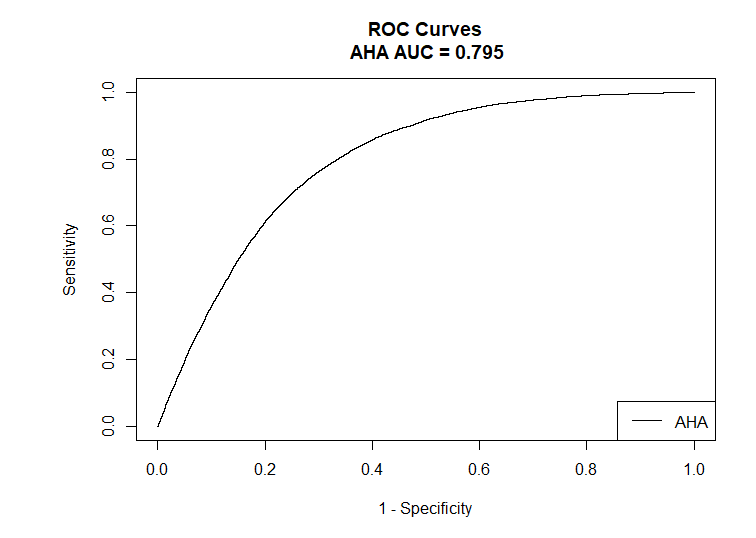
\includegraphics[width=8cm, height=8cm]{prelim-results/AHA/AHA_ROC.png}
   				\label{AHAROC}
   				\captionsetup{justification=justified,singlelinecheck=false,margin=1cm}
   				\caption{AHA/ACC 2013 ROC Curve, p-value < 0.001}
	   		\end{figure}
   		
   			\subsection{Clalit Model Population Flow Chart}
   			\begin{figure}[H]
	   			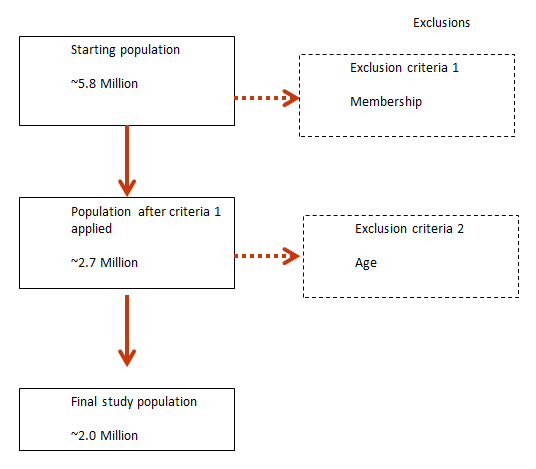
\includegraphics[width=10cm,height=8cm]{prelim-results/Panpredictor/pop_flow_chart.png}
	   			\captionsetup{justification=justified,singlelinecheck=false,margin=2cm}
	   			\caption{Population Flow Chart}
	   		\end{figure}
   		
   	\end{appendices}
	
\end{document}